\par Para calcular la absorción sonora se deben medir los tiempos de reverberación siguiendo el procedimiento de la Norma IRAM 4065/1995 \quotemarks{Acústica. Medición de absorción de sonido en sala reverberante}.

Durante el ensayo se utilizan 2 posiciones diferentes de las fuentes sonoras y 6 posiciones del micrófono, realizándose 3 registros por cada combinación fuente-micrófono. De este modo, cada tiempo de reverberación es el resultado del promedio de 36 caídas. Este procedimiento se lleva a cabo para dos condiciones: la cámara vacía y la cámara con la muestra ensayada en su interior, obteniéndose los resultados del cuadro~\tableref{tab:Tiempos_reverberacion}.


\begin{table}[H]
    \centering
    \begin{tabular}{|c|c|c|} \hline
        \textbf{Banda TR} & \textbf{Sala con muestra (T2)}& \textbf{TR Sala vacía (T1)} \\ \hline \hline
        100&	4,60&	14,92\\ \hline
        125&	4,47&	12,22 \\ \hline
        160&	3,71&	9,97 \\ \hline
        200&	3,20&	9,08 \\ \hline
        250&	2,89&	9,19 \\ \hline
        315&	2,72&	9,74 \\ \hline
        400&	2,38&	8,74 \\ \hline
        500&	2,28&	7,59 \\ \hline
        630&	2,26&	7,15\\ \hline
        800&	2,21&	7,03 \\ \hline
        1000&	2,28&	7,21 \\ \hline
        1250&	2,23&	6,58 \\ \hline
        1600&	2,21&	5,87 \\ \hline
        2000&	2,23&	5,08 \\ \hline
        2500&	2,22&	4,44 \\ \hline
        3150&	2,17&	3,59 \\ \hline
        4000&	2,08&	2,98 \\ \hline
        5000&	1,84&	2,29 \\ \hline
    \end{tabular}
    \caption{Tiempos de reverberación medidos, en seg}
    \label{tab:Tiempos_reverberacion}
\end{table}

\par En este caso, se desea clasificar la pantalla implementada de acuerdo a las categorías de la norma UNE-EN 1793-2: \quotemarks{Características intrínsecas relativas al aislamiento al ruido aéreo en condiciones de campo sonoro difuso}. Para ello, se calcula el número global:

\begin{equation}
        DL_\alpha = -10\cdot log \big( \frac{\sum_{i=1}^{18} 10^{0.1 \cdot L_i} \cdot \alpha_{si} }{\sum^{18}_{i=1} 10^{0.1 \cdot L_i} }\big)
    \label{eq:DL_a}
\end{equation}

\par Donde:
\begin{itemize}
    \item $\alpha_{si}$: Coeficiente de absorción sonora de la i-ésima banda de tercio de octava.
    \item $L_i$:Nivel de presión sonora de ruido normalizado ponderado A, en dB, de la iésima banda de tercio de octava del ruido normalizado ferroviario.
\end{itemize}

\par Para obtener los resultados de dicha ecuación, se necesitan los valores de relación de absorción sonora $\alpha$. Para obtener dicho valor, utilizamos nuevamente la expresión del área acústica equivalente del material, pero considerando ambos tiempos de reverberación como se muestra en la ecuación~\eqref{eq:area_equivalente_contiempos_reverberacion}:

\begin{equation}
    A_{iEq} = 55.3 \cdot \frac{V_{camara}}{C} \cdot (\frac{1}{TR_2} - \frac{1}{TR_1})
    \label{eq:area_equivalente_contiempos_reverberacion}
\end{equation}

\par Donde:
\begin{itemize}
    \item $V_{camara}$: En este caso $189m^3$.
    \item $C$: Velocidad del sonido a temperatura $26.7^\circ$. Entonces $C= 348.23 m/seg$.
    \item $TR_1$ y $TR_2$: Los tiempos de reverberación de la cámara vacía y con la muestra respectivamente.
\end{itemize}

\par A partir de este resultado, solo queda utilizar la relación :

\begin{equation}
    \alpha_{si} = A_{iEq} / S_{muestra};
\end{equation}

\par Donde $S_{muestra} = 10m^2$ es la superficie de muestra utilizada.\\


\par Podemos observar en la figura~\figref{fig::tiempos_reverberacion} como se comparan los tiempos de reverberación. Queda en evidencia, que el tiempo de reverberación en disminuye con la inclusión de la muestra en la sala y su efectividad disminuye a medida que aumenta la frecuencia.

\begin{figure}[H]
	\centering
	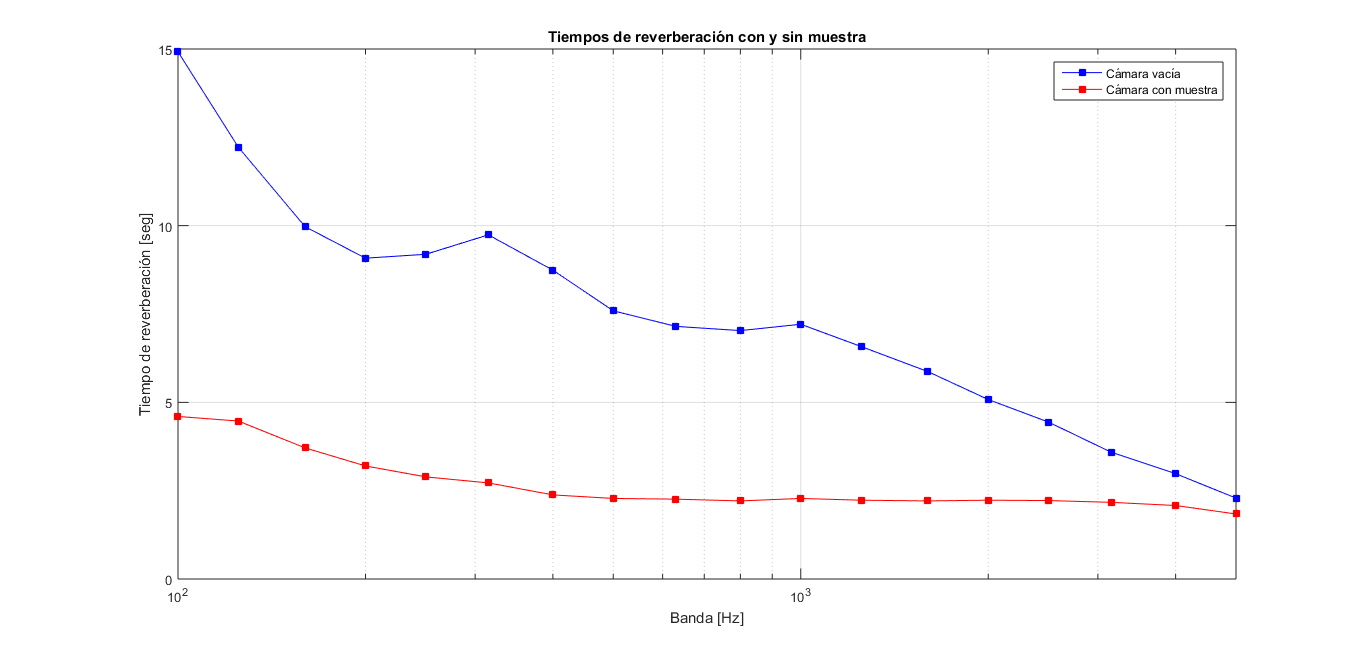
\includegraphics[scale=0.47]{./img/Tiempos_reverberacion.png}
	\caption{Tiempos de reverberación en la cámara reverberante}
	\label{fig::tiempos_reverberacion}
\end{figure}

\par Presentamos en el cuadro~\tableref{tab:coef_absorcion_sonora} y en la figura~\figref{fig::coef_absorcion_sonora} los resultados obtenidos mediante las mediciones.


\begin{table}[]
    \centering
    \begin{tabular}{|c|c|} \hline
        \textbf{Banda} & Coef Absorcion \\ \hline \hline
        100 & 45,13\\ \hline
        125	& 42,58\\ \hline
        160	& 50,79\\ \hline
        200	& 60,74\\ \hline
        250	& 71,19\\ \hline
        315	& 79,53\\ \hline
        400	& 91,77\\ \hline
        500	& 92,09\\ \hline
        630	& 90,83\\ \hline
        800	& 93,11\\ \hline
        1000&	90,01\\ \hline
        1250&	88,98\\ \hline
        1600&	84,68\\ \hline
        2000&	75,51\\ \hline
        2500&	67,60\\ \hline
        3150&	54,71\\ \hline
        4000&	43,58\\ \hline
        5000&	32,05\\ \hline
    \end{tabular}
    \caption{Coeficiente de absorción}
    \label{tab:coef_absorcion_sonora}
\end{table}


\begin{figure}[H]
	\centering
	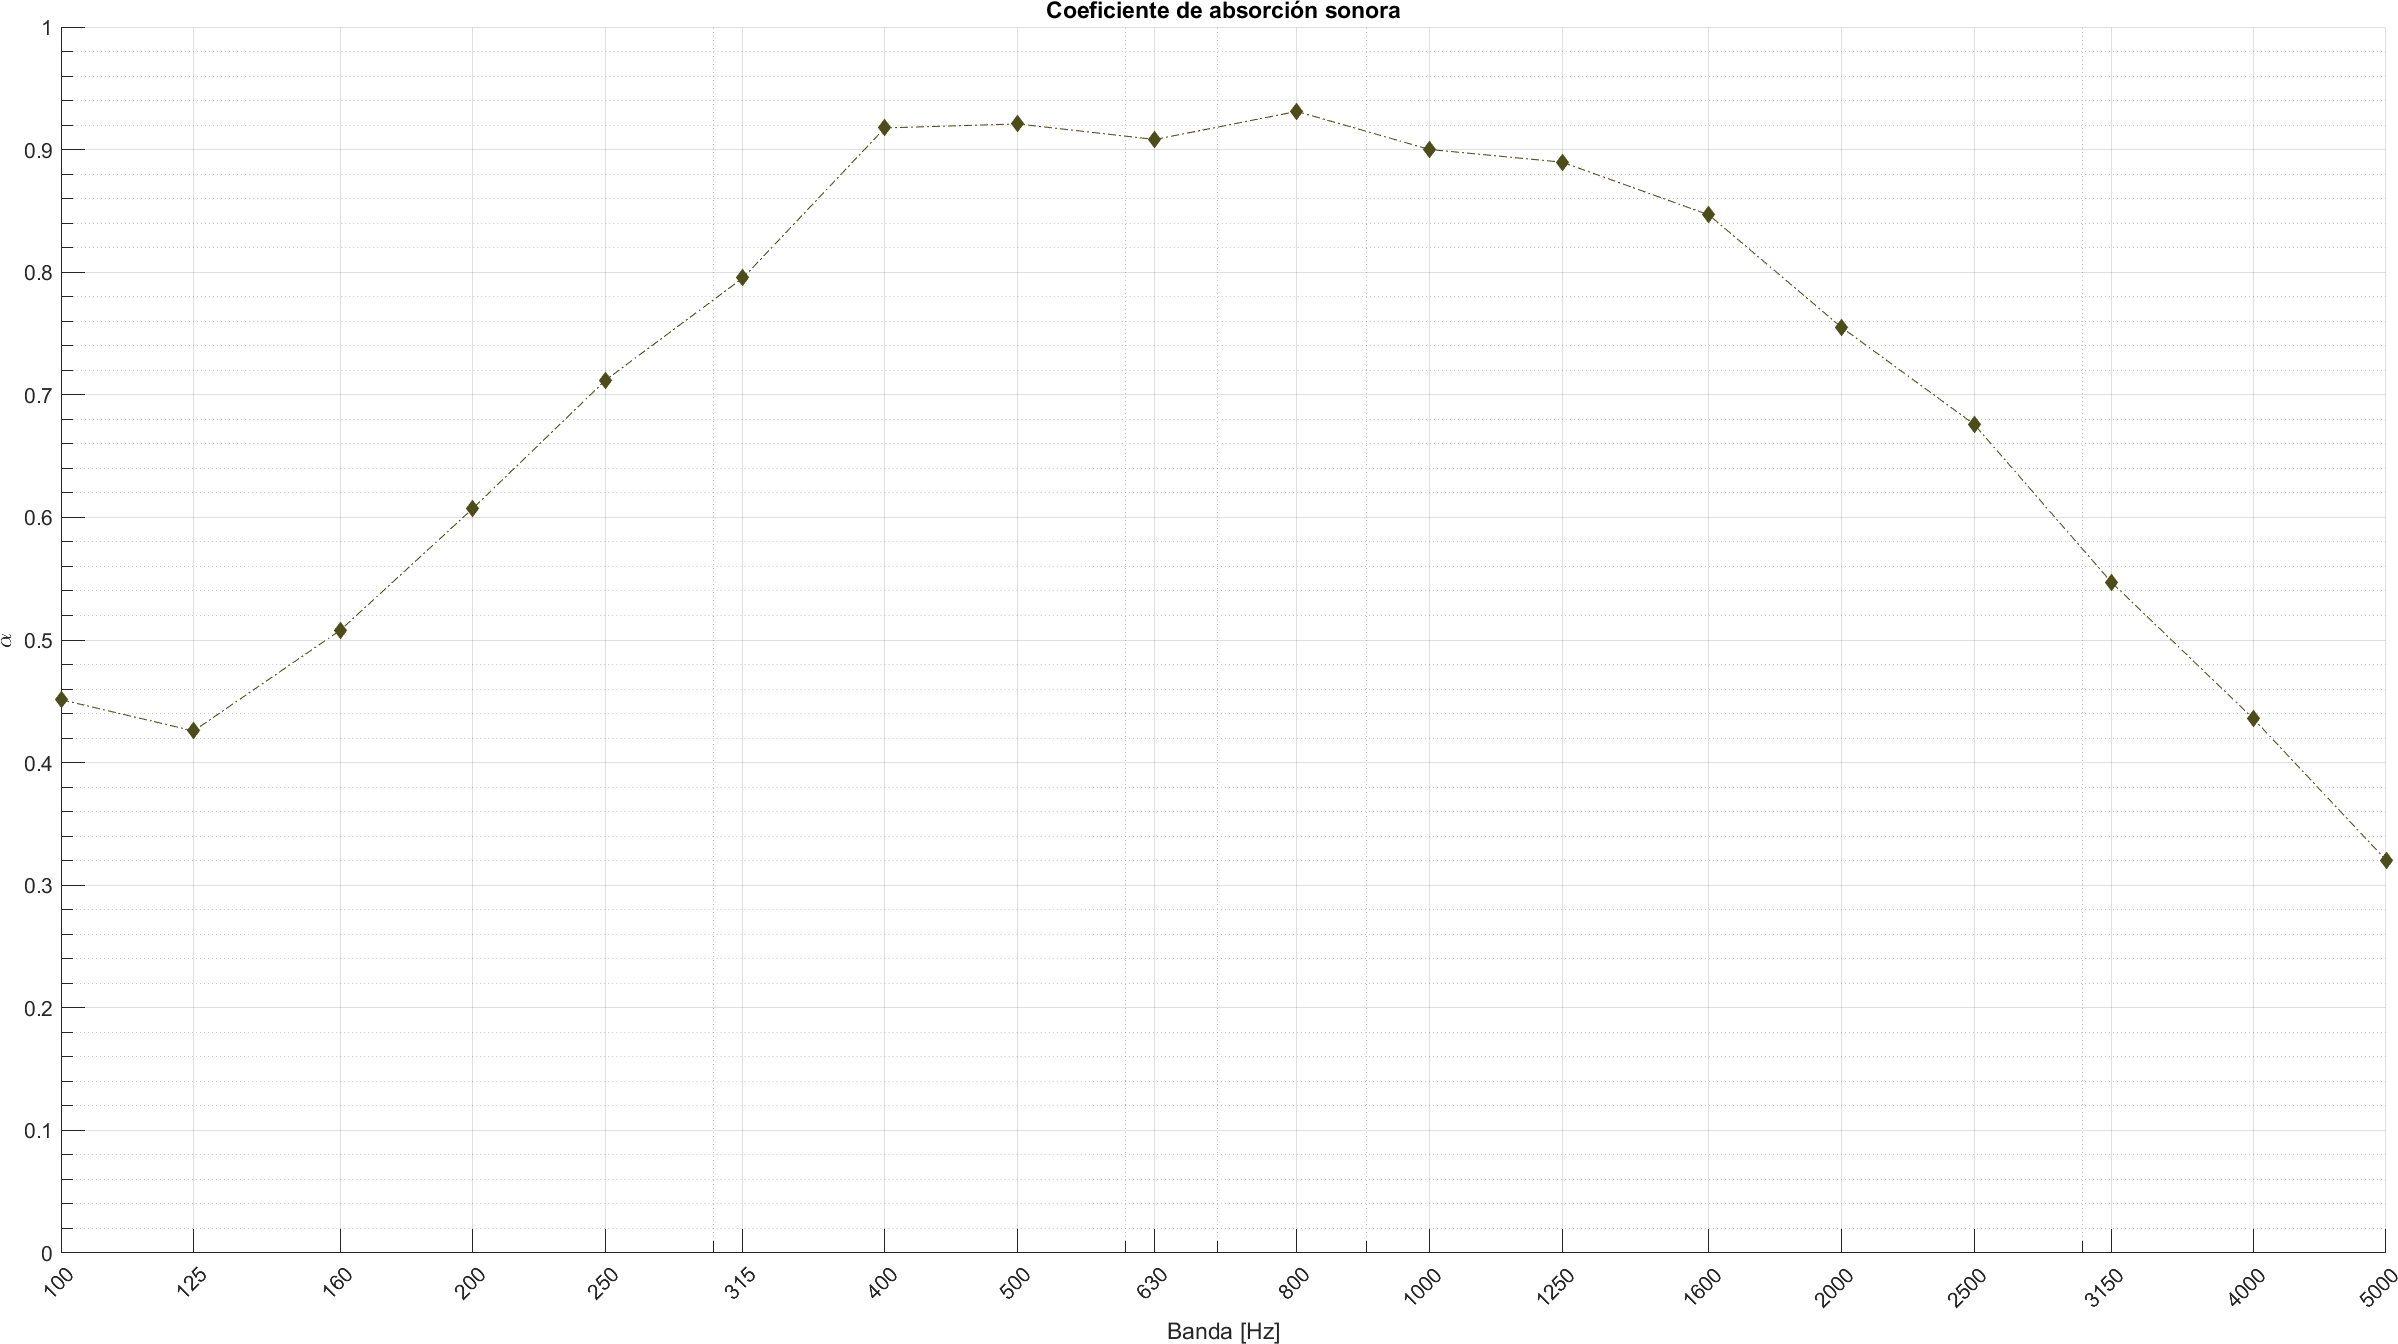
\includegraphics[scale=0.47]{./img/Coef_absorcion_sonora.png}
	\caption{}
	\label{fig::coef_absorcion_sonora}
\end{figure}

\par A partir de dichos resultados, podemos obtener el valor de evaluación:

\begin{equation}
    DL_{\alpha} =  6.4780 \approx 6
\end{equation}

\par Por lo tanto, podemos confirmar que el material cumple con la categoría $A_2$.


\begin{table}[H]
    \centering
    \begin{tabular}{|c|c|} \hline
        \textbf{Categoría} & \textbf{$DL_\alpha$ en dB} \\ \hline \hline
        A0& No determinado \\ \hline
        A1& $DL_\alpha < 4$ \\ \hline
        A2& 4 a 7 \\ \hline
        A3& 8 a 11 \\ \hline
        A4& 12 a 15 \\ \hline
        A5& $DL_\alpha >15$ \\ \hline
    \end{tabular}
    \caption{Caption}
    \label{tab:my_label}
\end{table}